% !TEX root = deckblatt3b.tex

\section{Invertierender Schmitt-Trigger}

In dieser Aufgabe war der Operationsverstärker als invertierender Schmitt-Trigger zu beschalten und dessen Funktionsweise zu erproben.\\

\subsection{Schaltung}

\begin{figure}[H]
  \begin{center}
    %\tikzset{component/.style={draw,thick,circle,fill=white,minimum size =0.75cm,inner sep=0pt}}
    \begin{circuitikz}
      \draw (-2,0)
      to[short] (-2,2)
      (-2,0) node[ground] (ground) {}
      (3,4) node[op amp] (opamp) {}
      (3,4.5) to[short] (3,5) node[vcc] {$V_{CC}$}
      (3,3.5) to[short] (3,3) node[ground] {}
      (opamp.-) to[short] (-2,4.5) to[short] (-2,4)
      (opamp.+) to[short] (1.8,2.3) to[short] (4.17,2.3) to[R=$R_1$] (4.17,0.5) 
	to[short] (-2,0.5) to[short] (7,0.5) to[short] (7,1.5) 
      (opamp.out) to[R=$R_2$] (4.17,2.5) to[short] (4.17,2)
      (opamp.out) to[short] (7,4) to[short] (7,3.5)
      ;
      \draw (1.8,2.3)
      to[R=$R_3$] (-0.5,2.3) to[short] (-1,2.3) to[voltage source,v>=$V_{CC}$] (-1,0.5)
      ;
       \draw (-2,3.5)
       to[short] (-2,3) node[vee] {};
      \draw (-2.5,3) node[] {$U_e$};
      \draw (7,3)
       to[short] (7,2.5) node[vee] {};
      \draw (7.5,2.5) node[] {$U_a$};
      \draw (3.5,2)
       to[short] (3.5,1.3) node[vee] {};
      \draw (3,1.5) node[] {$U_t$};
    \end{circuitikz}
    \caption{inververtierender Schmitt-Trigger}
  \end{center}
\end{figure}
\noindent

\begin{figure}[H]
 \begin{center}
  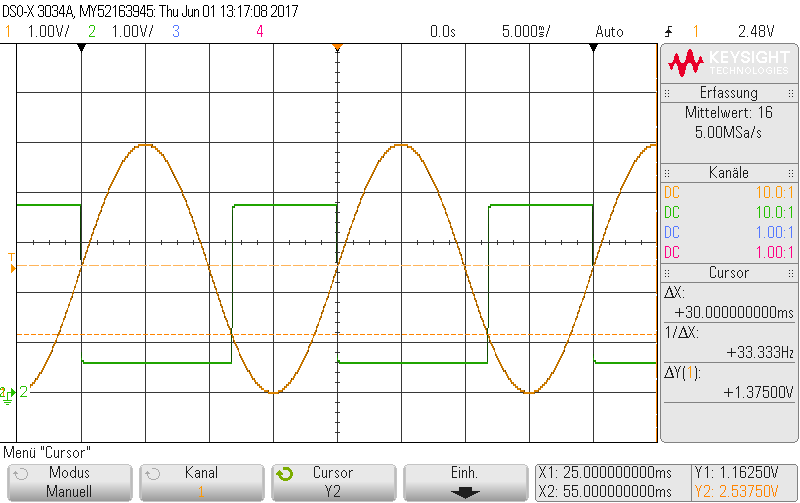
\includegraphics[height=6cm,width=12cm]{OsziBilder/SchmittTrigger_Time}
 \end{center}
 \caption{Zeitverlauf invertierender Schmitt-Trigger, $U_e$ orange und $U_a$ grün}
\end{figure}
\noindent
Der Schmitt-Trigger ist eine mitgekoppelte Operationsverstärkerschaltung. Seine Schaltschwellen liegen im allgemeinen symmetrisch
um den Nullpunkt. Durch das Anlegen einer Referenzspannung können die Schaltpunkte für das Über- bzw Untersteuern auch nicht 
symmetrisch angesetzt werden. Wird die positive Schaltschwelle erreicht, wird am Ausgang die negative Versorgungsspannung
des OPV's ausgegeben (hier $0V$, Masse). Wird die negative Schaltschwelle erreicht, wird die positive Versorgungsspannung 
ausgegeben (hier $V_{CC} = 5V$), diese wird allerdings nicht ganz erreicht, da es sich hier nicht um eine Rail-to-Rail OPV handelt.\\
\\
$U_e=$ Sinus $5V_{pp}$ $50Hz$ Offset $2,5V$, $V_{CC} = +5V$, $R_1=R_2=4,7k\Omega$, $R_3=10k\Omega$\\
gemessen: $U_a=3,18V$, $U_t=1,72V$\\

\subsection{Hysterese}

\begin{figure}[H]
 \begin{center}
  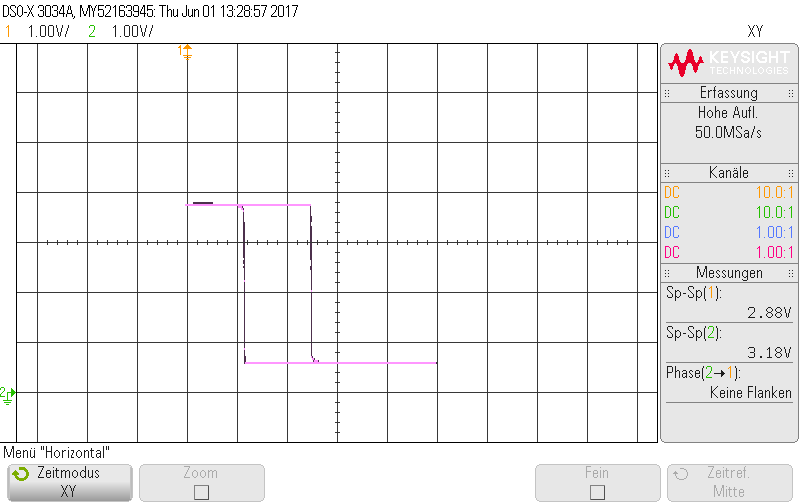
\includegraphics[height=6cm,width=12cm]{OsziBilder/SchmittTrigger_XY}
 \end{center}
 \caption{Hysterese-Kennlinie, x-Achse $U_e$, y-Achse $U_a$}
\end{figure}
\noindent
Die Hysterese-Kennlinie zeigt die Schaltpunkte des Triggers, diese werden durch den von der 
Ausgangsspannung beeinflussten Spannungsabfall am Widerstand $R_1$ verschoben. Die aus der Simulation 
berechneten Schaltpunkte sind, $U_{low}=0,963V$ und $U_{high}=2,728V$. Diese sind auch mit kleinen
Abweichungen in der Kennlinie zu erkennen, $U_{low}\approx 1,1V$ und $U_{high}\approx 2,25V$.\\
\\
Der Schmitt-Trigger wird zur digitalisierung von Signalen eingesetzt. Eine Hysterese wird hierbei benötigt, 
da an den Schaltflanken oft Störsignale ein mehrfaches Über- bzw. Untersteuern des Operationsverstärkers verursachen, was
zu falschen Codierungen führen kann.
